\documentclass{article}[12pt]

\usepackage[utf8]{inputenc}
\usepackage[margin=1in]{geometry}
\usepackage{amsmath}
\usepackage{amsfonts}
\usepackage{amssymb}
\usepackage{bm}
\usepackage{graphicx}
\usepackage{url}
\usepackage{caption}
\usepackage{subcaption}
\usepackage[numbib,nottoc]{tocbibind}

\title{A Longitudinal Analysis of the Synchronized Brainwave Dataset}
\author{Thomas Edwards and Jonathan Skaza}
\begin{document}
\maketitle
\begin{abstract}
This study applies methods from longitudinal data analysis to analyze the effect of two different audio-visual stimuli on brain wave activity. To summarize neurological activity, the study considers two aggregate measures, attention and meditation, which emphasize beta and alpha waves, respectively. To gain insight into the stimulus effect, we implement both univariate and multivariate analyses under a mixed model framework. Results support the notion that the two stimuli have differing effects on the levels of attention and meditation, indicating that certain audio-visual stimuli may be leveraged to manipulate brain wave activity. 
\end{abstract}
\section{Introduction}

Discovering the secret to advancing one's mental capabilities has been a desire by many researchers over the years. Brainwave entrainment, or `brainwave synchronization', is a phrase coined by scientists to represent the brain's ability to balance both hemispheres, allowing them to work in sync. This phenomenon of syncing one's brain waves is currently being linked to theories that explain how the brain is capable of changing thoughts or making well-educated decisions in the blink of an eye. As referenced by some, it would seem impractical for the system of electrical impulses in the brain to constantly make new connections only to break them apart, ``[t]here's got to be some way of dynamically establishing circuits to correspond to the thoughts we're having in this moment, and then if we change our minds a moment later, those circuits break apart somehow. We think synchronized brain waves may be the way the brain does it'' \cite{trafton}. 

Recent developments in brainwave-sensing devices have allowed investigators to perform experiments in order to tackle the challenge of better understanding our neurological functions. Specifically, MIT researchers published an article in 2014 that claims ``synchronized brain waves enable rapid learning'' \cite{trafton}. In the study, they examine electroencephalogram (EEG) data collected on monkeys attempting to learn how to assign proper dots into one of two corresponding categories.  Their primary objective was to determine if the observed neurological pattern in the monkeys ``reflects communication between the prefrontal cortex and striatum, or if each region is working independently'' \cite{trafton}. Analysis on the EEG patterns illustrates a development of synchronization among ‘beta bands’ as the monkeys learned the categories. Lead investigator, Earl Miller, describes this behavior as a ‘humming’ of circuits that ``may then foster subsequent long-term plasticity changes in the brain, so real anatomical circuits can form'' \cite{trafton}. As it was the first of its kind, this analysis marked a breakthrough in linking particular patterns of synchrony with specific thoughts \cite{trafton}. Furthermore, the study demonstrates that the prefrontal cortex uses an iterative process to allow for constant modifications as the brain receives new information, explaining how humans are able to maintain an open-ended nature of thought.

It is important to understand the functionality behind each type of brain wave before diving deeper into the principles of brainwave entrainment. Brain waves are divided into four main groups known as ‘brain states': beta (13-29.75 Hz), alpha (7.5-12 Hz),  theta (3.5-6.75 Hz), and delta (0.5-2.75 Hz) waves. Each wave type is associated with an activity or state-of-being. In beta state, the mind is fully awake and attentive. As the brain transitions from beta to alpha state, the mind relaxes and focuses more on intrapersonal qualities. Upon falling asleep, individuals enter the subconscious mind primarily associated with theta state. In theta state, one has access to spontaneous insights in the form of dreams.  Diving into a deep sleep opens the door to the delta state of mind where the body has a chance to recover and rejuvenate.
In general, lower frequency brain waves are associated with inward attention while higher frequencies are associated with outward focus. To analyze this, investigators use EEG, which is the study of  changing electrical frequencies within the brain. In this present study, it is the means to discovering potential ways of syncing together the frequencies of the various waves \cite{Giorgio}.  

The purpose of this study is to use longitudinal EEG data to investigate how different stimuli impact synchronization of brain activity. We utilize a mixed model approach to evaluate the effect that each stimulus has on specified brain wave frequency over time.  For sake of simplicity, we use NeuroSky's eSense meters for attention and meditation as representative outcomes to summarize brain activity.  Possible confounders relating to the subjects' experience with the stimuli are incorporated into the modeling as well.  The results of the analysis are intended to provide insight into how one's brain waves can be manipulated in order to maintain a synchronized neurological state so that cognitive function is optimized. With such knowledge, further steps can be taken within the field of public health to improve upon methods designed for mentally-impaired individuals, who could stand to drastically benefit from brainwave synchronization. We proceed to introduce our methodological approach before presenting the results of the longitudinal analysis. We conclude with a discussion regarding the interpretation, public health impact, and limitations of our results.


\section{Methods}

The data used in this study were obtained from \textit{Kaggle}, a popular data science website.
The experiment involved thirty students from the MIDS class at UC Berkeley School of Information \cite{data}. Each student was randomly assigned to one of two sessions. Each session presented a slightly different audio-visual 5-minute stimulus video. Both stimuli instructed the participants to: blink eyes five times; close eyes, relax, clear mind of distractions, and focus on breathing for 30 seconds; perform multiple mental algorithmic calculations; close eyes, relax, listen to music; watch Doritos ad; close eyes and think of items that relate to a given category; and silently count the number of rectangles of a chosen color from a series of images. The music, mental calculations, Doritos ad, categories, and images were different in each of the two stimuli. Consumer-grade EEG devices were used to collect brainwave patterns on the subjects as they were presented the stimuli. 

The dependent variables of interest are standardized values from 0 to 100 that represent attention and meditation levels. The study was unbalanced, meaning that each subject, $i$, had $n_i$ distinct attention and meditation measurements. The primary predictor of interest is an interaction between stimulus (i.e., session) and time. Available controls include gender, whether or not the participants had previously seen the Doritos ad, whether or not the participants saw the hidden icons displayed during the color counting exercise, and the chosen color for the color counting exercise. The final dataset includes all of the subjects’ readings before, during, and after the stimulus presentation. In total, the dataset consists of 30,013 readings, an average of about 1,000 per participant.

\begin{figure}
	\centering
	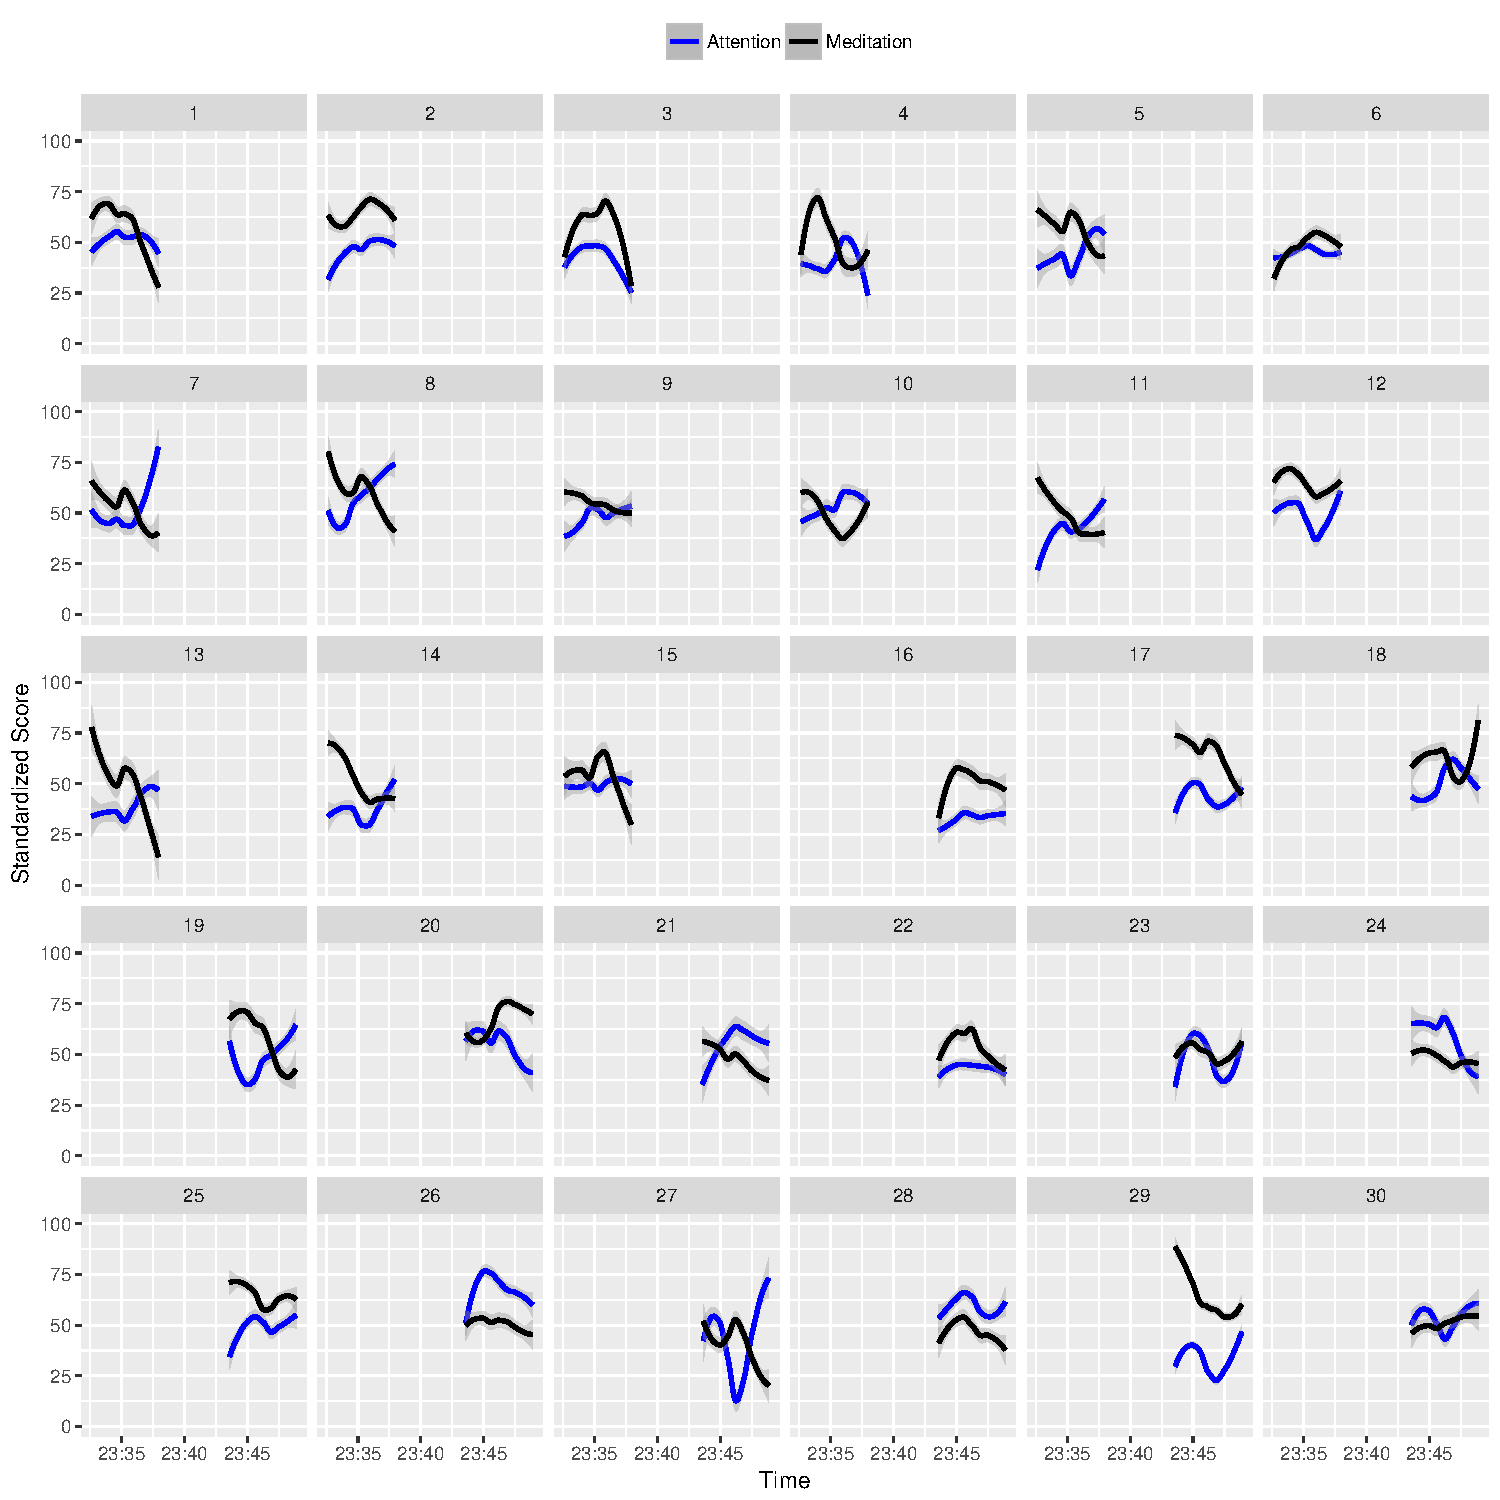
\includegraphics[width=\linewidth]{figures/traj.pdf}
	\caption{Smoothed Attention and Meditation trajectories by subject.}
	\label{fig:traj}
\end{figure}

However, not all observations were relevant to the present analysis. Seeing that our main interest is the effect of the stimuli on current neurological activity, readings taken before and after the stimulus videos were discarded. 
%Furthermore, we deemed it appropriate to remove all observations with signal quality larger than 127. Signal quality values greater than 127 indicate that the EEG headset was not being worn properly, potentially contaminating the readings. 
A summary of the number of repeated measures for each subject (i.e., $n_i$) before and after data cleaning can be found in Table~\ref{tab:meta}. Moreover, Figure~\ref{fig:traj} contains LOESS curves which describe the attention and meditation trajectories for each subject throughout the duration of the study.  Figure~\ref{fig:dist} contains histograms of attention and meditation scores taken from the entire study. It is evident that, when aggregated, both attention and meditation scores are approximately normally distributed.

% latex table generated in R 3.2.3 by xtable 1.8-2 package
% Mon Dec 12 12:02:27 2016
\begin{table}[ht]
\centering
\begin{tabular}{rrr}
  \hline
 & Raw & Clean \\ 
  \hline
Min. & 464.00 & 308.00 \\ 
  1st Qu. & 624.25 & 320.00 \\ 
  Median & 1067.00 & 321.00 \\ 
  Mean & 1000.43 & 331.80 \\ 
  3rd Qu. & 1266.75 & 321.75 \\ 
  Max. & 1607.00 & 644.00 \\ 
   \hline
\end{tabular}
\caption{Summary statistics for number of repeated measures, $n_i$, before
                  and after data cleaning.} 
\label{tab:meta}
\end{table}


\begin{figure}[h]
	\centering
	\begin{minipage}{.45\textwidth}
		\centering
		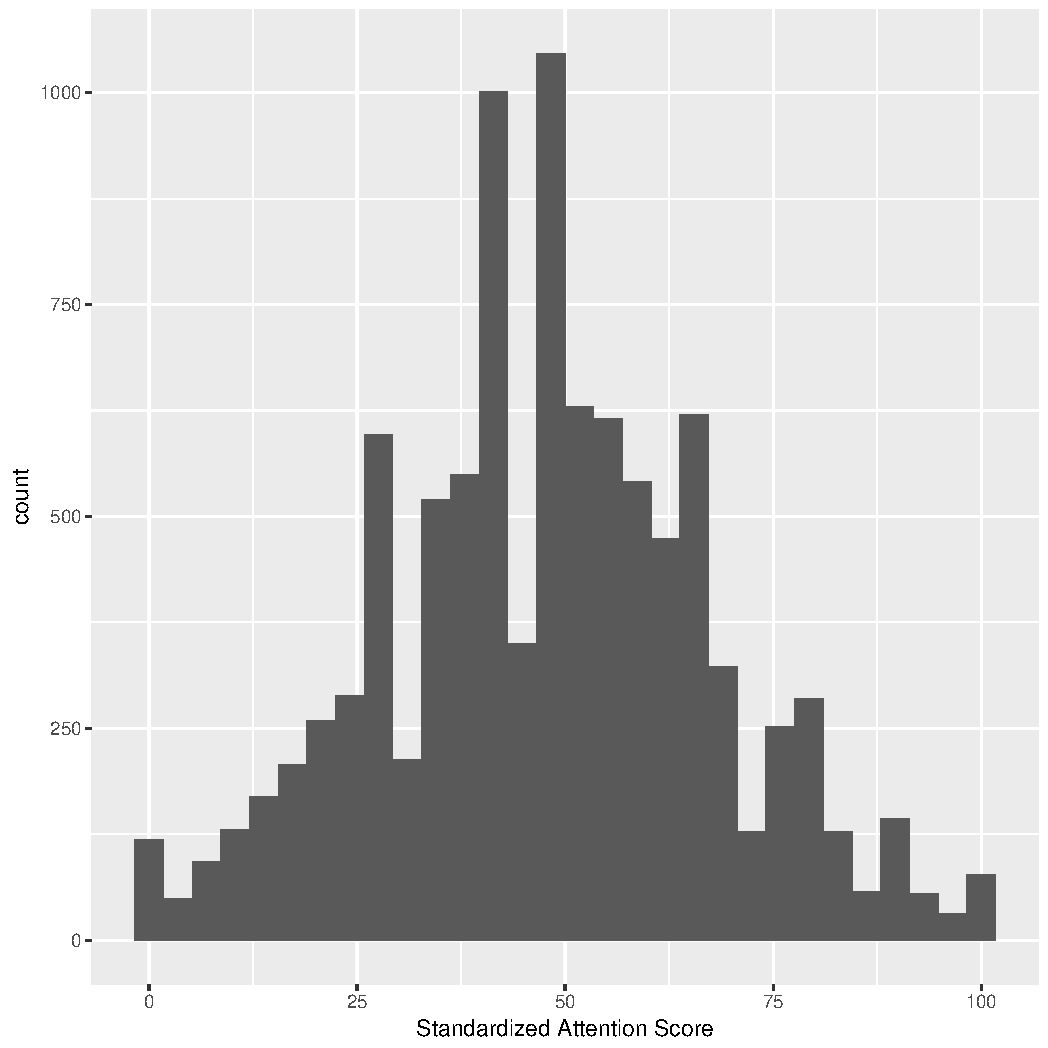
\includegraphics[width=0.9\linewidth]{figures/dista.pdf}
	\end{minipage}
	\begin{minipage}{0.45\textwidth}
		\centering
		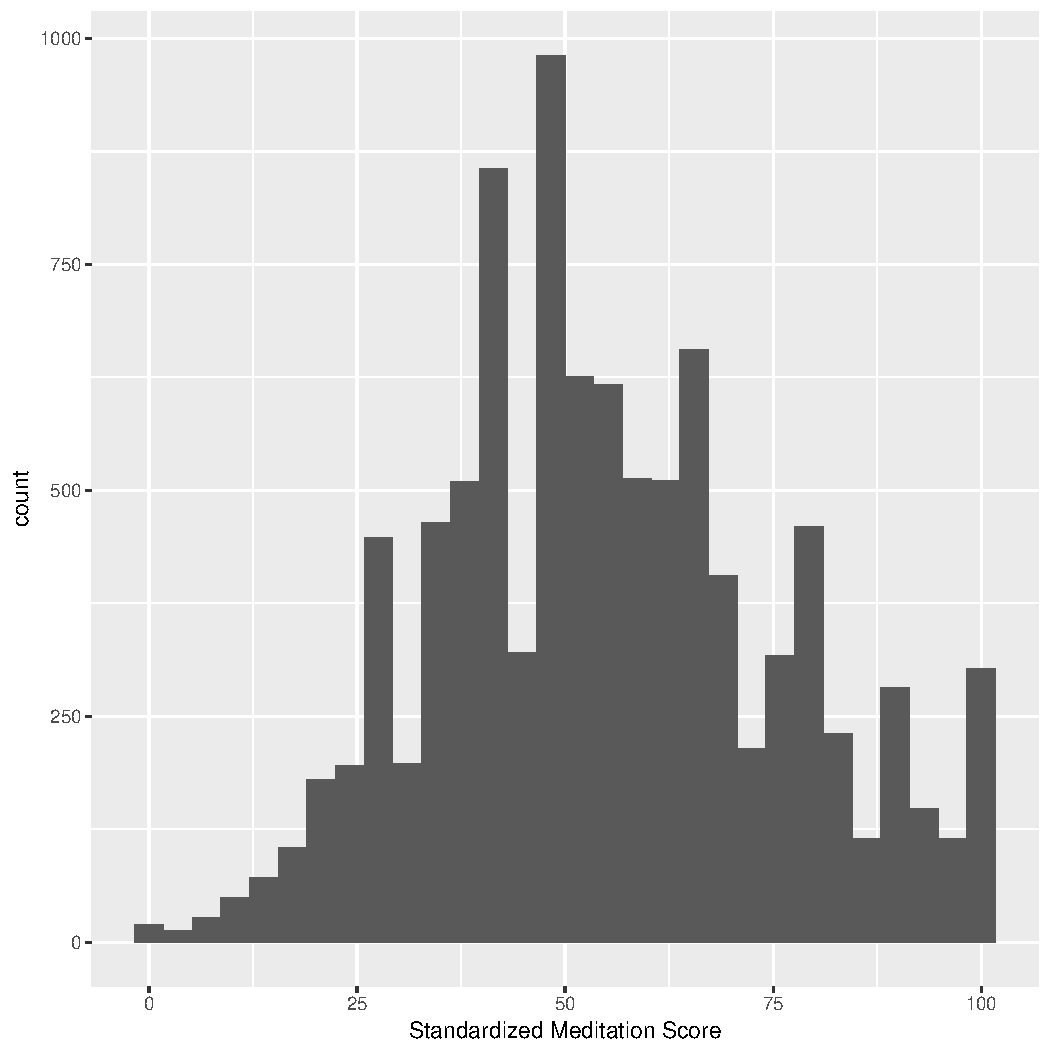
\includegraphics[width=0.9\linewidth]{figures/distm.pdf}
	\end{minipage}
	\caption{Distributions of the attention scores and meditation scores for all subjects throughout the duration of the stimuli.}
	\label{fig:dist}
\end{figure}


We followed a two-step approach in analyzing the effect of variables on both attention and meditation levels. We first implemented a univariate analysis, effectively treating the two outcomes as independent of one another. In this stage of the analysis, we formulated and estimated linear mixed effects models for each outcome. Subsequently, we carried out a bivariate analysis, taking the correlation between attention and meditation into consideration, by specifying and estimating a multivariate linear mixed effects model.\footnote{The correlation between attention and meditation was $-0.141$ in the clean dataset.}

The intent of the univariate analysis was to assess the relationship between attention level and covariates and meditation level and covariates under the assumption that attention level and meditation level are independent. To do so, we formulated the following linear mixed effects models,
\begin{align}
\mathbf{Y_{1i}} = \mathbf{X_{i}} \boldsymbol{\beta_{1}} + \mathbf{Z_{i}} \boldsymbol{b_{1i}} \label{att}
+ \boldsymbol{\epsilon_{1i}} \\
\mathbf{Y_{2i}} = \mathbf{X_{i}} \boldsymbol{\beta_{2}} + \mathbf{Z_{i}} \boldsymbol{b_{2i}}
+ \boldsymbol{\epsilon_{2i}} \label{med}
\end{align}
where $\mathbf{Y_{1i}}$ and $\mathbf{Y_{2i}}$ are $(n_i \times 1)$ vectors containing the repeated attention and meditation levels for the $i^{th}$ subject, respectively, $\mathbf{X_{i}}$ is a $(n_i \times 19)$ matrix of covariates, $\mathbf{Z_{i}}$ is a $(n_i \times 1)$ vector of 
$\left(\begin{array}{c c c c}
1 & 1 & \dots & 1
\end{array}\right)^T$, $\boldsymbol{\beta_{1}}$ is a $(19 \times 1)$ vector of fixed effects corresponding to Equation~\ref{att}, $\boldsymbol{\beta_{2}}$ is a $(19 \times 1)$ vector of fixed effects corresponding to Equation~\ref{med}, $\boldsymbol{b_{1i}}$ is a scalar representing a random intercept in Equation~\ref{att}, and $\boldsymbol{b_{2i}}$ is a scalar representing a random intercept in Equation~\ref{med}.\footnote{$\mathbf{X_{i}}$ and $\mathbf{Z_{i}}$ are identical in both models.} $\boldsymbol{\epsilon_{1i}}$ and $\boldsymbol{\epsilon_{2i}}$ are included as error terms. We used Restricted Maximum Likelihood (REML) to obtain estimates for $\boldsymbol{\beta_{j}}$ and $\boldsymbol{b_{ji}}$ for $j = 1,2$. The computation was performed using the \texttt{lmer} package in R  \cite{lme4}.

As mentioned above, the main objective of the modeling is to assess whether there is a significant interaction between stimulus (i.e., session) and time. A result supporting this notion would indicate that different parts of the stimulus videos have distinct effects on attention and/or meditation levels. For instance, we attempt to answer questions such as the following: \textit{Does the color counting exercise in session 1 have the same effect on meditation levels as it does in session 2?}. Since both stimuli were organized identically, we made use of spline terms to answer these questions more precisely. The time effect is allowed to vary with session and the mental exercise within that session. In practice, this coincides with breaking each session into five distinct parts, which we refer to as calculations, music, ad, categories, and colors.

In the bivariate analysis, we formulated and subsequently estimated the following multivariate linear mixed model,

\begin{align}
\left(\begin{array}{c}
\mathbf{Y_{1i}} \\
\mathbf{Y_{2i}}
\end{array}\right)
= \mathbf{X^\prime_{i}} 
\left(\begin{array}{c}
\boldsymbol{\beta_{1}} \\
\boldsymbol{\beta_{2}}
\end{array}\right)
+
\mathbf{Z_{i}} 
\left(\begin{array}{c}
\boldsymbol{b_{1i}} \\
\boldsymbol{b_{2i}}
\end{array}\right)
+
\left(\begin{array}{c}
\boldsymbol{\epsilon_{1i}} \\
\boldsymbol{\epsilon_{2i}}
\end{array}\right)
\end{align}

The notation is similar to that above except the model is estimated jointly, taking the correlation between the two responses into account. Additionally we replace $\mathbf{X_{i}}$  with $\mathbf{X^\prime_{i}}$.  $\mathbf{X^\prime_{i}} $ is simply a subset of $\mathbf{X_{i}}$. We included fewer covariates in the multivariate model---eliminating the insignificant predictors of color chosen and icon status ---to ensure a more parsimonious model. To obtain estimates, we utilized the \texttt{MCMCglmm} package in R \cite{mcmc}. The package uses Markov chain Monte Carlo (MCMC) routines to fit multi-response generalized linear mixed models. MCMC methods provide an alternative strategy for marginalizing the random effects that may be more robust than other techniques \cite{zhao06}. Unlike the univariate linear mixed model---in which each parameter estimated is linked with a test-statistic---we determine ``significance'' in the multivariate analysis using a quantity referred to as pMCMC. If testing $\beta_j$, then pMCMC can be interpreted as follows,
\begin{align}
	2*\min\{Pr(\beta_j < 0), Pr(\beta_j > 0)\}
\end{align}
where the probabilities are obtained from the MCMC simulation.



\section{Results}

The results from the univariate analysis are presented in Table~\ref{tab:att} and Table~\ref{tab:med}. The most noteworthy results revolve around the interactions between the spline terms and stimulus group (session). Generally speaking, the spline-session interactions are highly significant, providing evidence of differing attention and meditation responses over time between the stimuli presented in the two videos. Additionally, gender is a significant predictor of attention after adjusting for other covariates, with females demonstrating significantly higher levels of attention than males.

% latex table generated in R 3.2.3 by xtable 1.8-2 package
% Mon Dec 12 12:02:27 2016
\begin{table}[ht]
\centering
\begin{tabular}{rrrr}
  \hline
 & Estimate & Std. Error & t value \\ 
  \hline
(Intercept) & 55.93 & 4.20 & 13.33 \\ 
  genderm & -11.07 & 4.07 & -2.72 \\ 
  seen.video.beforey & 8.74 & 4.12 & 2.12 \\ 
  saw.iconsy & -3.77 & 3.02 & -1.25 \\ 
  colorg & -5.52 & 3.75 & -1.47 \\ 
  colorr & -8.85 & 4.14 & -2.14 \\ 
  colory & -2.89 & 7.72 & -0.37 \\ 
  time & -0.28 & 0.04 & -7.64 \\ 
  time.calculations & 0.87 & 0.07 & 11.76 \\ 
  time.music & -1.00 & 0.08 & -12.02 \\ 
  time.ad & 0.68 & 0.08 & 8.38 \\ 
  time.categories & -0.34 & 0.06 & -5.29 \\ 
  time.colors & 0.14 & 0.03 & 3.98 \\ 
  time:session2 & 0.55 & 0.05 & 11.20 \\ 
  time.calculations:session2 & -1.19 & 0.10 & -11.81 \\ 
  time.music:session2 & 1.04 & 0.12 & 9.02 \\ 
  time.ad:session2 & -0.74 & 0.11 & -6.56 \\ 
  time.categories:session2 & 0.34 & 0.09 & 3.82 \\ 
  time.colors:session2 & -0.01 & 0.05 & -0.28 \\ 
   \hline
\end{tabular}
\caption{Results from the linear mixed effects model
             with attention as the response.} 
\label{tab:att}
\end{table}


% latex table generated in R 3.2.3 by xtable 1.8-2 package
% Mon Dec 12 12:02:27 2016
\begin{table}[ht]
\centering
\begin{tabular}{rrrr}
  \hline
 & Estimate & Std. Error & t value \\ 
  \hline
(Intercept) & 48.89 & 3.78 & 12.93 \\ 
  genderm & 4.72 & 3.64 & 1.30 \\ 
  seen.video.beforey & -8.85 & 3.68 & -2.40 \\ 
  saw.iconsy & -3.26 & 2.70 & -1.21 \\ 
  colorg & 4.53 & 3.36 & 1.35 \\ 
  colorr & 2.87 & 3.70 & 0.78 \\ 
  colory & -4.45 & 6.90 & -0.64 \\ 
  time & 0.47 & 0.04 & 12.44 \\ 
  time.calculations & -1.26 & 0.08 & -16.50 \\ 
  time.music & 1.44 & 0.09 & 16.72 \\ 
  time.ad & -1.20 & 0.08 & -14.41 \\ 
  time.categories & 0.73 & 0.07 & 11.05 \\ 
  time.colors & -0.33 & 0.04 & -9.32 \\ 
  time:session2 & -0.13 & 0.05 & -2.70 \\ 
  time.calculations:session2 & 0.41 & 0.10 & 3.96 \\ 
  time.music:session2 & -0.48 & 0.12 & -4.02 \\ 
  time.ad:session2 & 0.36 & 0.12 & 3.13 \\ 
  time.categories:session2 & -0.27 & 0.09 & -2.90 \\ 
  time.colors:session2 & 0.20 & 0.05 & 4.01 \\ 
   \hline
\end{tabular}
\caption{Results from the linear mixed effects model
             with meditation as the response.} 
\label{tab:med}
\end{table}


The results from the multivariate linear mixed model, presented in Table~\ref{tab:bivariate}, are consistent with those from the univariate analysis. Again, 9 out of a possible 10 spline-session interaction terms  are significant, while gender has a significant effect on attention levels. More thorough interpretations of the effects of interest obtained from the multivariate model follow.

% latex table generated in R 3.2.3 by xtable 1.8-2 package
% Mon Dec 12 00:11:18 2016
\begin{table}[ht]
\centering
\begin{tabular}{rrrrrr}
  \hline
 & post.mean & l-95\% CI & u-95\% CI & eff.samp & pMCMC \\ 
  \hline
traitattention & 41.79 & 37.79 & 45.78 & 1000.00 & 0.00 \\ 
  traitmeditation & 52.98 & 49.01 & 56.26 & 1000.00 & 0.00 \\ 
  at.level(trait, 1):genderf & 6.35 & -0.20 & 13.26 & 1000.00 & 0.07 \\ 
  genderf:at.level(trait, 2) & -2.10 & -8.28 & 4.02 & 1000.00 & 0.48 \\ 
  at.level(trait, 1):seen.video.beforey & 6.30 & -1.84 & 13.95 & 1000.00 & 0.12 \\ 
  at.level(trait, 2):seen.video.beforey & -6.88 & -13.87 & 0.74 & 1195.27 & 0.06 \\ 
  at.level(trait, 1):time & -0.28 & -0.35 & -0.20 & 1000.00 & 0.00 \\ 
  at.level(trait, 2):time & 0.47 & 0.40 & 0.54 & 1000.00 & 0.00 \\ 
  at.level(trait, 1):time.calculations & 0.87 & 0.72 & 1.02 & 1000.00 & 0.00 \\ 
  at.level(trait, 2):time.calculations & -1.25 & -1.40 & -1.11 & 1000.00 & 0.00 \\ 
  at.level(trait, 1):time.music & -1.00 & -1.17 & -0.84 & 1000.00 & 0.00 \\ 
  at.level(trait, 2):time.music & 1.43 & 1.27 & 1.60 & 1000.00 & 0.00 \\ 
  at.level(trait, 1):time.ad & 0.68 & 0.53 & 0.85 & 1000.00 & 0.00 \\ 
  at.level(trait, 2):time.ad & -1.20 & -1.36 & -1.04 & 1000.00 & 0.00 \\ 
  at.level(trait, 1):time.categories & -0.34 & -0.46 & -0.22 & 1000.00 & 0.00 \\ 
  at.level(trait, 2):time.categories & 0.73 & 0.61 & 0.85 & 1000.00 & 0.00 \\ 
  at.level(trait, 1):time.colors & 0.14 & 0.07 & 0.20 & 1150.45 & 0.00 \\ 
  at.level(trait, 2):time.colors & -0.33 & -0.41 & -0.27 & 1000.00 & 0.00 \\ 
  at.level(trait, 1):time:session2 & 0.54 & 0.43 & 0.64 & 1000.00 & 0.00 \\ 
  at.level(trait, 2):time:session2 & -0.12 & -0.23 & -0.04 & 1000.00 & 0.01 \\ 
  at.level(trait, 1):time.calculations:session2 & -1.18 & -1.40 & -0.99 & 1000.00 & 0.00 \\ 
  at.level(trait, 2):time.calculations:session2 & 0.39 & 0.20 & 0.59 & 1000.00 & 0.00 \\ 
  at.level(trait, 1):time.music:session2 & 1.04 & 0.80 & 1.26 & 1000.00 & 0.00 \\ 
  at.level(trait, 2):time.music:session2 & -0.47 & -0.71 & -0.25 & 1000.00 & 0.00 \\ 
  at.level(trait, 1):time.ad:session2 & -0.74 & -0.97 & -0.52 & 1000.00 & 0.00 \\ 
  at.level(trait, 2):time.ad:session2 & 0.36 & 0.15 & 0.58 & 1000.00 & 0.00 \\ 
  at.level(trait, 1):time.categories:session2 & 0.34 & 0.18 & 0.52 & 1000.00 & 0.00 \\ 
  at.level(trait, 2):time.categories:session2 & -0.27 & -0.43 & -0.07 & 1000.00 & 0.00 \\ 
  at.level(trait, 1):time.colors:session2 & -0.01 & -0.11 & 0.07 & 1000.00 & 0.77 \\ 
  at.level(trait, 2):time.colors:session2 & 0.20 & 0.11 & 0.30 & 1000.00 & 0.00 \\ 
   \hline
\end{tabular}
\caption{Results from the bivariate
               linear mixed effects model. at.level(trait,1) refers to attention while 
               at.level(trait,2) corresponds to meditaion.} 
\label{tab:bivariate}
\end{table}


\newpage
\subsection{Relevant Interpretations}

\noindent After adjusting for gender and whether or not the individual has seen the Doritos ad prior to the experiment, given the subject's intercept, every 1 second increase in time is associated with a(n): 
\begin{itemize}
\item Increase in attention score of 0.54 standard units for subjects watching the beginning relaxation section of stimulus 2 compared to stimulus 1.
\item Decrease in meditation score of 0.12 standard units for subjects watching the beginning relaxation section of stimulus 2 compared to stimulus 1.
\item Decrease in attention score of 0.64 standard units for subjects performing the calculations of stimulus 2 compared to stimulus 1.
\item Increase in meditation score of 0.27 standard units for subjects performing the calculations of stimulus 2 compared to stimulus 1.
\item Increase in attention score of 0.41 standard units for subjects listening to music from stimulus 2 compared to stimulus 1.
\item Decrease in meditation score of 0.20 standard units for subjects listening to music from stimulus 2 compared to stimulus 1.
\item Decrease in attention score of 0.34 standard units for subjects watching the Doritos ad shown in stimulus 2 compared to stimulus 1.
\item Increase in meditation score of 0.16 standard units for subjects watching the Doritos ad shown in stimulus 2 compared to stimulus 1.
\item Approximately no change in attention score for subjects thinking of objects that fit into given categories specified by stimulus 2 compared to stimulus 1.
\item Decrease in meditation score of 0.11 standard units for subjects thinking of objects that fit into given categories specified by stimulus 2 compared to stimulus 1.
\item Approximately no change in attention score for subjects counting colors of block illustrations displayed by stimulus 2 compared to stimulus 1.
\item Increase in meditation score of 0.09 standard units for subjects counting colors of block illustrations displayed by stimulus 2 compared to stimulus 1.
\end{itemize}

The clear inverse relationship between attention and meditation levels over time supports the theory that the correlation between the two outcomes is negative. This seems to be consistent with the literature, since high attention level corresponds with brain waves predominantly in beta state where the frequencies are between 13 to 27 Hz. In contrast, high meditation level corresponds to a mind in alpha state where frequencies range from 7 to 12 Hz. Thus,  it is expected an increase in one score will lead to a decrease in the other.

\section{Discussion}

Both the univariate and multivariate models are consistent in the sense that the exercises presented in each of the two stimuli have a significant association with attention and meditation levels over time for subjects similar to the ones in the study.  The significance of the spline terms indicate that even small differences in tasks that one is asked to accomplish can lead to considerable differences in brain activity.  These results suggest that visual stimuli can be utilized to alter one's brainwaves in a synchronized fashion. Further investigation of exact methods that can hold the mind in a state of meditation or attention could be beneficial. In particular,
``[d]uring meditation, the grand central station-like cable of nerves connecting your two brain hemispheres, the Corpus Callosum --- becomes deeply stimulated, much like a joggers legs on a long run'' \cite{infinisync}.  Routinely meditating correctly is much like exercising in that it strengthens the mind and allows individuals to ``tap into a whole range of extraordinary abilities they never knew they had'' \cite{infinisync}. Thus, incorporating daily meditation with the aid of an appropriate stimulus into people's everyday lives could serve as a next step from a public health perspective.  The impact this could have could be particularly beneficial for individuals who suffer from anxiety, depression, or other mental illnesses. According to one estimate, it takes just 25 minutes of meditation to balance out the brainwaves of both hemispheres allowing them to work in sync, thereby optimizing mental and emotional health \cite{infinisync}.

We recognize that certain features of the experimental design and our analysis might have influenced the outcome values, limiting inferences that may be drawn. First, the two groups of participants did not watch the stimulus videos simultaneously. Session 2 participants had to wait about 30 minutes for session 1 participants to prepare and watch their stimulus video before entering and participating. It is difficult to determine if/how this `resting' phase before being exposed to the stimulus influenced the EEG readings for group 2. Although we include a random intercept term in our model to account for all discrepancies between individuals at the beginning of the stimulus video, this time gap might still generate biased results. Another limitation worth noting is the small sample size of 30 subjects (and only 7 females). A larger and more representative sample size would make inferences more stable and generalizable.

However, even  with a more representative sample, we should not expect to discover neurological techniques that apply to everyone.  Human brain activity is a heterogeneous process and it would be difficult to imagine a stimulus that affects every unique individual in a similar way. We feel that the most logical approach would be to develop methods that are known to work well on specific subgroups of people.  Methodology similar to that utilized by precision medicine studies would make for a useful template in how to design future experiments.  Additions to this template design include, but are not limited to:
having a baseline control group consisting of EEG data collected on subjects that do not watch any stimulus video,
constructing a matched pairs design to reduce variability since brainwave data are so heterogeneous,
and adding tasks such as physical exercise, jump scares, games, etc. to obtain a better understanding of how a wider array of activities affects brainwave synchronization.
EEG technology has the power and potential to provide substantive insight into cognitive capabilities, indicating that well-designed future studies and carefully constructed analyses are warranted.




\bibliographystyle{plain}
\bibliography{bibliography}

\end{document}
